%\documentclass[12pt,openright,twoside,openany]{report}
\documentclass[12pt]{report}
\usepackage[utf8]{inputenc}
\usepackage[a4paper, total={6in, 10in}]{geometry}

%\usepackage [french]{babel}
\usepackage{xspace}
\usepackage[dvipsnames]{xcolor}
\usepackage{graphicx}
\usepackage{url}
\usepackage{caption}
\usepackage{subcaption}
\usepackage{parskip}
\usepackage{wrapfig}
%\usepackage{hyperref}

\title{
{\LARGE \textbf{ Projet de Programmation \\ Génération procédurale de planètes }}\\
 {\large Master 1 }\\
 {\vspace{10mm}}
 {
\includegraphics[width=0.6\textwidth]{images/télécharger.png}}
 }
 \author{\textbf{Professeur accompagnant:} M. Mansencal\\\textbf{Cahier des besoins rédigé par:} \\Alexey Zhukov, Tony Wolff, Baptiste Bedouret, \\Alexis Marec, Antoine Fredefon, Thomas Mercier}

\date{02/03/2022}

\makeatletter
\def\@makechapterhead#1{%
  \vspace*{5\p@}%
  {\parindent \z@ \raggedright \normalfont
    \ifnum \c@secnumdepth >\m@ne
      \if@mainmatter
        %\huge\bfseries \@chapapp\space \thechapter
        \Huge\bfseries \thechapter.\space%
        %\par\nobreak
        %\vskip 20\p@
      \fi
    \fi
    \interlinepenalty\@M
    \Huge \bfseries #1\par\nobreak
    \vskip 40\p@
  }}
\makeatother

\begin{document}

\maketitle
\clearpage

\vspace*{\stretch{1}}
\tableofcontents
\vspace*{\stretch{1}}
\newpage

\chapter{Introduction et objectifs du projet}

% Faire une intro sur le développement des algos de génération procédurale, et surtout sur l'importance de l'optimisation de ceux-ci pour le rendu temps-réel (jeux-vidéo, simulation).

La génération procédurale de planètes est un problème complexe qui requiert des compétences dans des domaines variés, notamment pour modéliser la sphère avec des niveaux de détails variables en fonction de la résolution demandée. Dans le cadre de ce projet, la carte de hauteur de la planète sera générée au vol par un ou plusieurs algorithmes conseillés par le sujet. Cette carte, couramment appellée heightmap, représente en chaque point la distance séparant un sommet et le centre de la planète. Notre première étape consiste donc à trouver, comprendre et utiliser une bibliothèque pour générer des heightmaps de manière procédurale. La principale difficulté de cette étape sera de génerer des cartes sphériques simulant la surface d'une planète.

Dans un second temps, notre objectif sera de créer une bibliothèque permettant le stockage de la heightmap d'une planète en utilisant les principes de niveau de détail (Level of Detail ou LOD). En effet, les algorithmes de LOD permettent de sauvegarder les cartes dans différents niveaux de précision que nous pouvons contrôler. Les algorithmes que nous allons étudier puis mettre en oeuvre permettront alors de stocker la heightmap de manière optimale pour faire du LOD, c'est à dire réguler la quantité de sommets à tracer selon la distance entre le maillage et l'observateur.

Enfin, dans le but d'afficher la planète, nous devrons développer un outil de visualisation simple utilisant la bibliothèque OpenGL. En plus de donner un aperçu de la planète (et donc de la qualité de la heightmap générée), cet outil permettra à l'utilisateur de se déplacer dans la scène pour faire apparaître les différents niveaux de détail de la surface.

Dans l'ensemble, cet outil permettra de générer la carte de hauteur d'une planète de manière procédurale, de la stocker dans une structure adaptée pour effectuer du LOD, et enfin de la visualiser dans une fenêtre OpenGL comme nous pouvons le voir sur la figure 1.1 et 1.2. 


\vspace{0.3cm}

 \begin{figure}[h]
\centering
\begin{center}
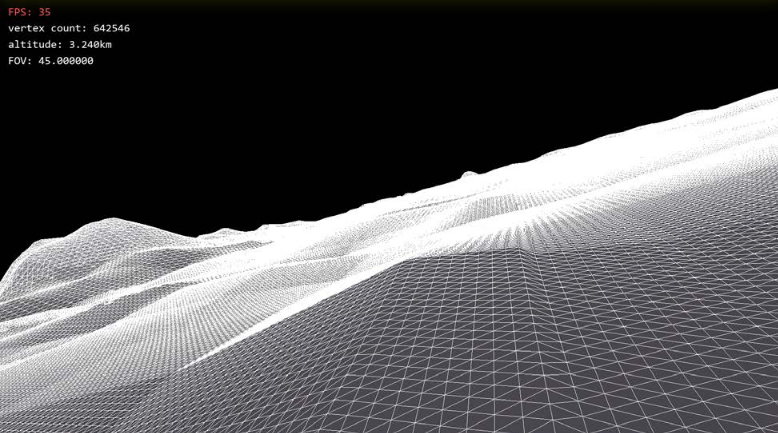
\includegraphics[scale = 0.4]{images/Capture d’écran du 2022-03-05 15-46-04.png}
\caption{Exemple de visualisation de la surface de la lune}
\source{https://dept-info.labri.fr/~narbel/PdP/Subjects21-22/CLOD-Planets/Planet_Rendering.pdf}
\end{center}
\end{figure}

\begin{figure} [ht]
  \centering
  \begin{center}
  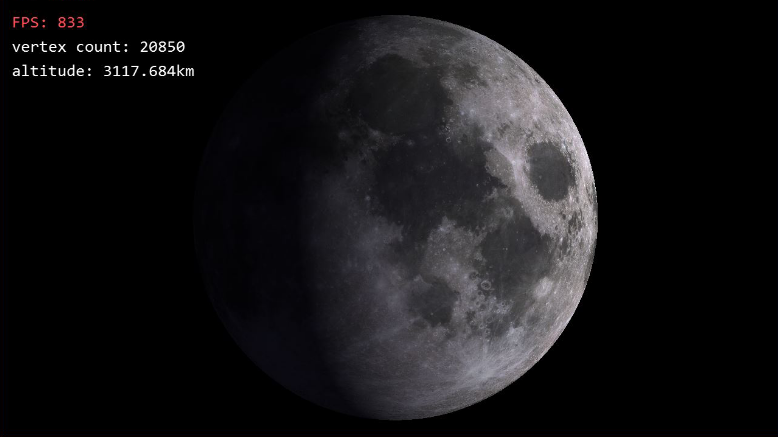
\includegraphics[scale = 0.4]{images/Capture d’écran du 2022-03-14 22-35-11.png}
  \caption{Exemple de visualisation de la surface de la lune}
  \source{https://dept-info.labri.fr/~narbel/PdP/Subjects21-22/CLOD-Planets/Planet_Rendering.pdf}
  \label{fig:gliederung}
  \end{center}
\end{figure}

\newpage

\chapter{Analyse de l'existant}

\section{Bibliothèque de génération de bruit}

Une bibliothèque de génération de bruit sera utile pour la création d'une heightmap 2D du moins. Définisson le terme : Une carte de hauteur est une image 2D monochrome. La valeur du pixel s'interprète comme la distance du terrain par rapport au sol, une valeur élevée se traduit par du blanc sur l'image, une valeur basse par des nuances de noirs, le noir total étant le niveau de la mer. Ces cartes sont créés soit à la main par des artistes, soit par des données de cartes déjà existantes, ou bien par des algorithmes de génération de bruit (notre solution).

\begin{enumerate}
    \item Libnoise
    Bibliothèque C++ de production de bruit "cohérent", bruit à variation régulière (classe de bruit dont font partie Perlin et Simplex). Comme indiqué sur la page web \cite{libnoisewebsite}, elle a déjà été utilisée sciemment dans le cas de la création d'une carte 2D pour une planète quelconque. 
    
    \begin{figure}[h]
    \centering
    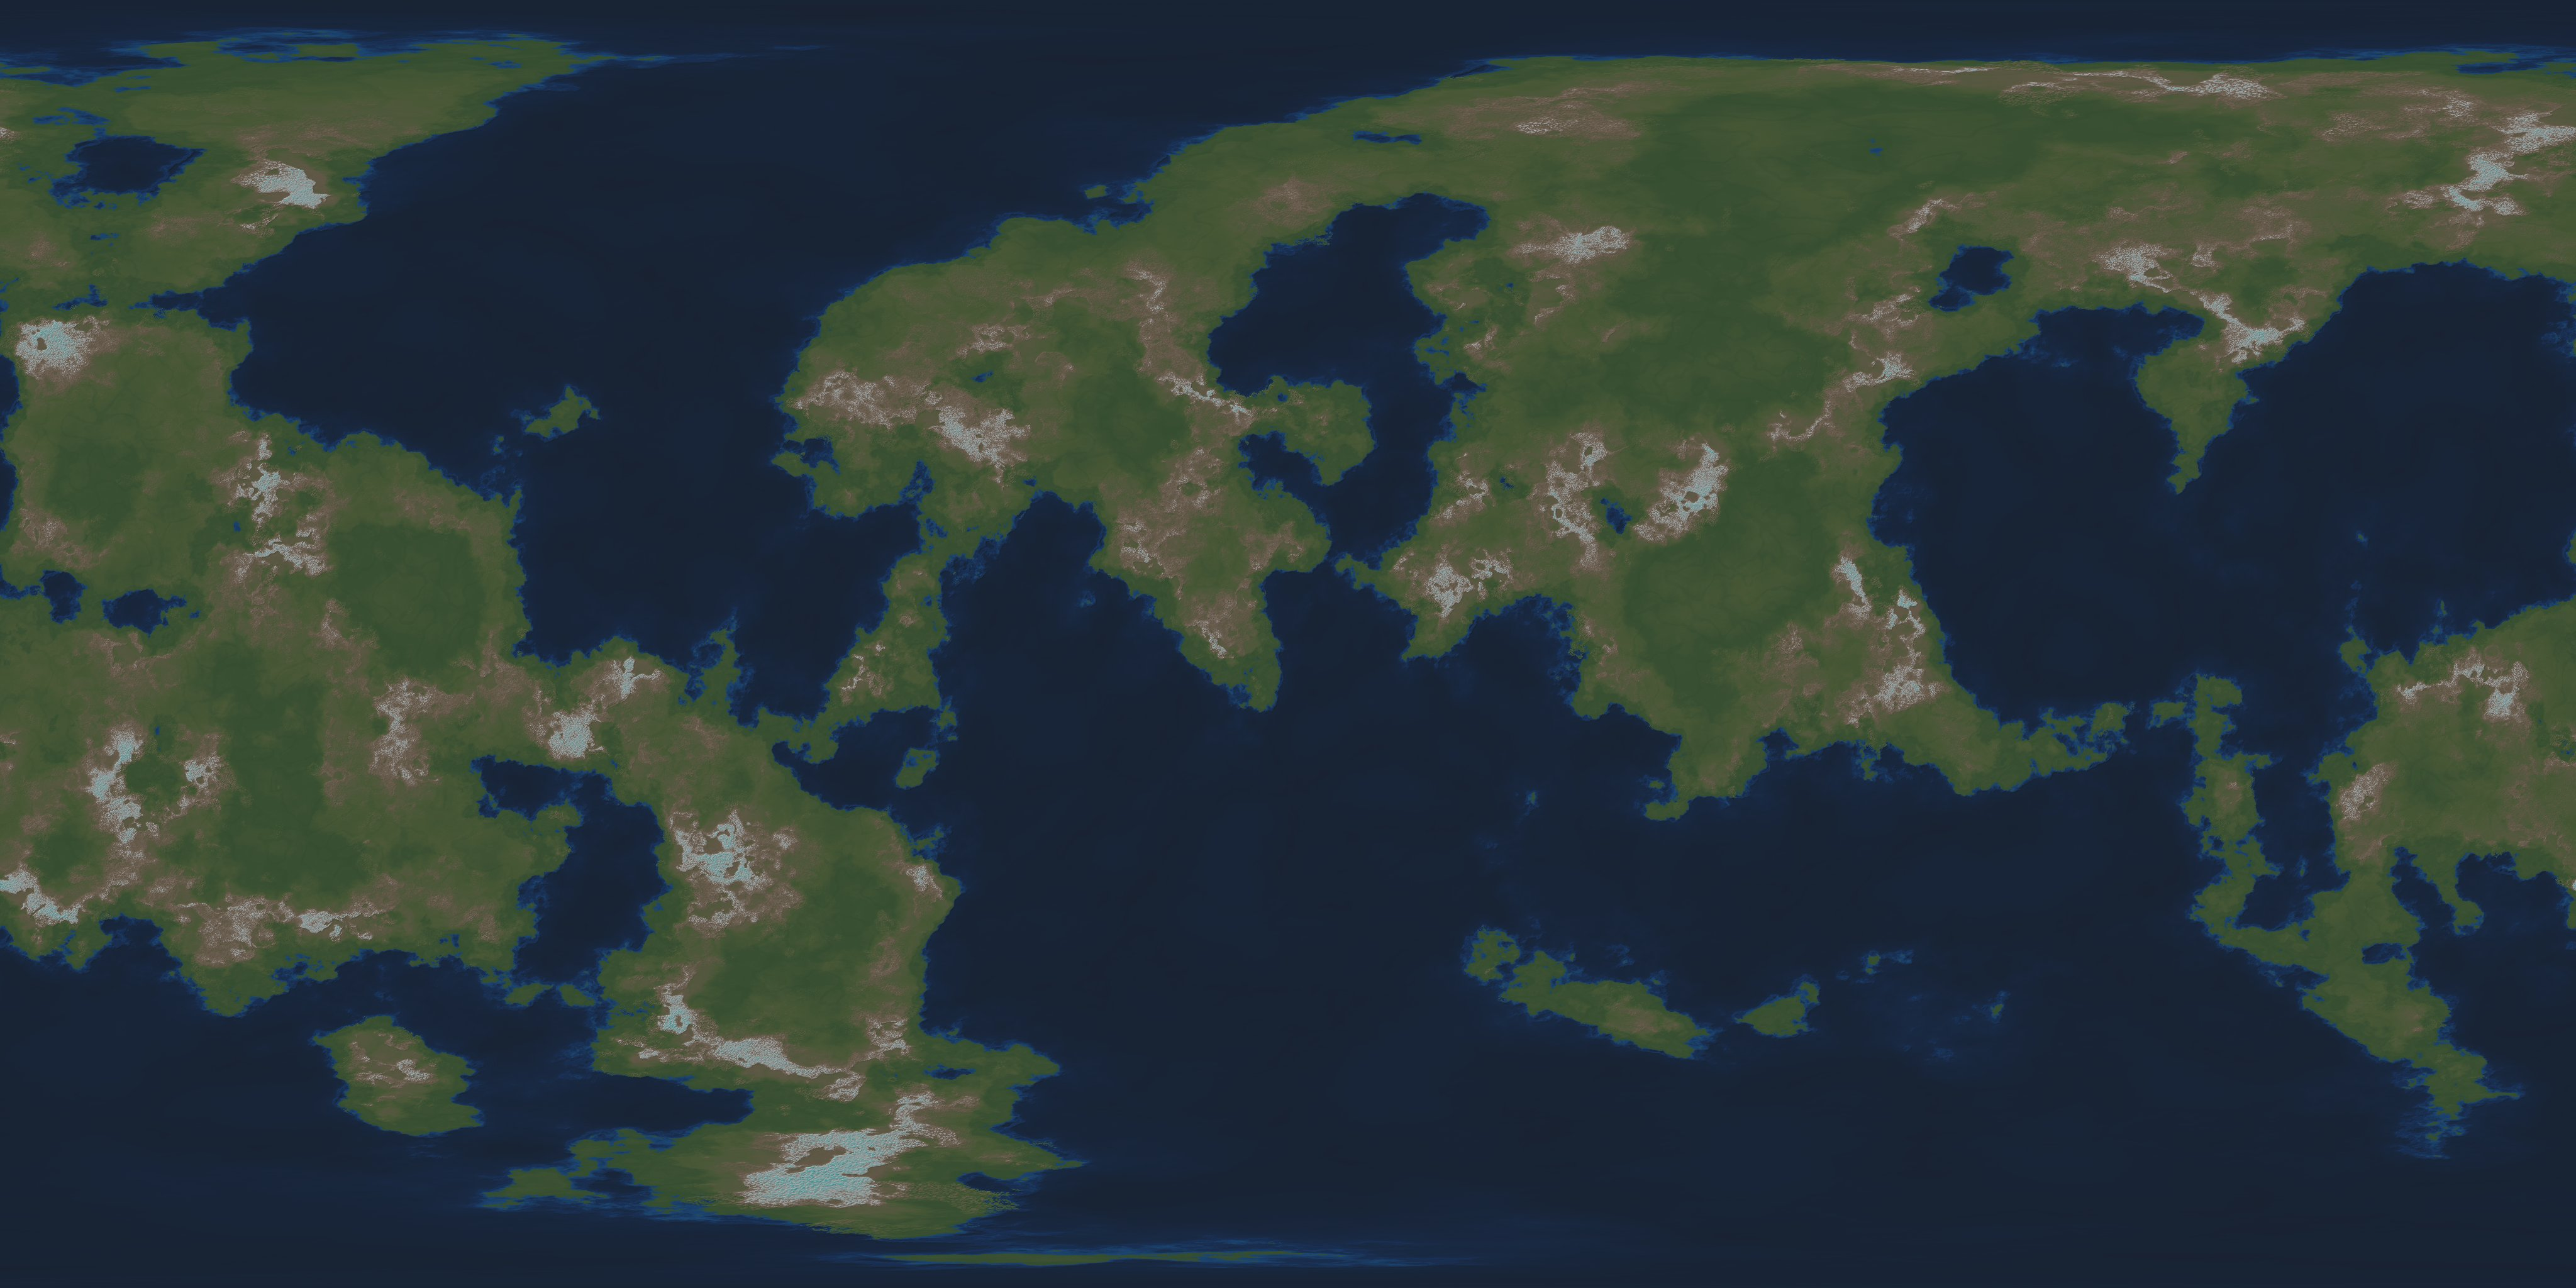
\includegraphics[scale = 0.05]{images/planet.jpg}
    \caption{texture d'une planète}
    \source{http://libnoise.sourceforge.net/examples/complexplanet/index.html}
    \end{figure}
 
    Elle précise bien que ce n'est pas un outil de rendu et qu'il faudra utiliser une autre bibliothèque ou notre propre code pour générer une image, elle propose l'utilisation de \textbf{noiseutils} qui sauve le désagrément décrire des classes telles que le remplissage de noise map (tableau 2D qui a vocation à recevoir les valeurs générées par les modules de bruit), des builders associés à ces noise map pour des objets mathématiques utiles comme la sphère dans notre cas, des classes pour sérialiser une image ou une noise map, et des classes pour créer des images bien entendu. 
     \newline D'après la documentation, un bruit "cohérent" respecte trois critères :
    \begin{enumerate}
        \item Si l'on passe la même valeur d'entrée, on obtient toujours la même valeur de sortie.
        \item Un petit changement dans la valeur d'entrée produira un petit changement dans la valeur de sortie.
        \item Un changement important de la valeur d'entrée produira un changement aléatoire de la valeur de sortie.
    \end{enumerate}
    
    \begin{figure}[h]
        \centering
        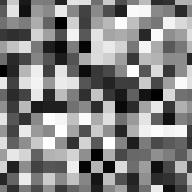
\includegraphics[scale = 0.5]{images/continuousintnoise2d.png}
        \caption{texture 2D obtenu à l'aide de la fonction continue de bruit cohérent}
    \end{figure}
    
    Elle part d'une fonction pseudo-random tel que \textit{rand()}. en C++ et prend en paramètres des entiers (ou réel pour la version continue), et renvoyant une entier entre -1 et 1, c'est \textit{integerNoise}.
    
    Pour éviter les froissements dans la texture, l'interpolation des valeurs entières se présente comme immanquable pour avoir des transitions douces entre valeurs de bruit. L'interpolation linéaire est une première version simple mais ne suffit pas à créer une niveau de détail naturel, alors la fonction de bruit cohérent va chercher à utiliser une version non linéaire, couplé à l'interpolation de vecteurs gradient à la place des valeurs entières de bruit. Le vecteur gradient est obtenu avec \textit{integerNoise} qui le sélectionne aléatoirement dans un ensemble de vecteurs précalculés. On utilisera la version 2D de cette fonction, chaque dimension correspond à un paramètre (2 dimensions égal à deux paramètres).
    Note : un ensemble de fonctions de bruits "cohérents" sera indispensable pour avoir l'essence d'une texture terrain, cette ensemble de fonction se retrouve dans le bruit de Perlin ou de Simplex.
    
     \begin{figure}[h]
        \centering
        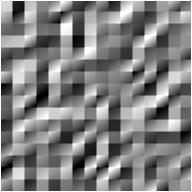
\includegraphics[scale = 0.7]{images/bumpvalue.png}
        \caption{bumpmap "froissée"}
    \end{figure}
    
    \begin{figure}[h]
        \centering
        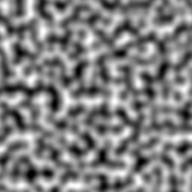
\includegraphics[scale = 0.5]{images/gradientcoherentnoise2d.png}
        \caption{texture 2D avec vecteur gradient}
    \end{figure}
    
\end{enumerate}

\newpage

\section{Algorithmes de niveau de détail}

Étant donnée l'importance de l'optimisation pour le rendu temps-réel, il existe de nombreuses approches abordant le problème du stockage et du rendu de heightmaps. La technique la plus couramment utilisée à l'heure actuelle se base sur des algorithmes de niveaux de détail (Level Of Detail ou LOD) pour subdiviser le maillage de la sphère en fonction de la distance au sol de l'observateur.

Dans un premier temps, nous avons étudié l'article de Filip Strugar \textit{Continuous Distance-Dependent Level of Detail for Rendering Heightmaps}\textbf{\cite{FStrugar}}. Bien que paru en 2010, cet article permet de comprendre plus en détail comment représenter une heightmap sous forme de quadtree (arbre quaternaire dont les particularités sont expliquées plus bas) et ainsi utiliser cette structure de données pour créer l'algorithme de rendu de heightmaps CDLOD.

Un quadtree ou arbre quaternaire est un arbre dont chaque noeud dispose au maximum de quatre enfants. Cette représentation est particulièrement utile pour effectuer une subdivision d'un espace en deux dimensions. En effet, une image 2D par exemple peut être partitionnée en quatre quadrants de tailles égales, comprenant chacun l'information de ce quart d'image. Puis, chaque quadrant peut être lui aussi subdivisé en quatre, et ainsi de suite tant que des éléments peuvent être distingués dans celui-ci. Le critère sera le nombre maximum de triangles autorisés dans un quadrant . La valeur maximale sera fixée à 10 000, de sorte que chaque quadrilatère continuera à être divisé jusqu'à ce qu'il contienne moins de 10 000 triangles.  Un bon moyen de visualiser le processus de création d'un quadtree est l'application interactive \textbf{quadtreevis}\footnote{https://jimkang.com/quadtreevis/}, permettant de visualiser la division de l'image de base ainsi que les noeuds de l'arbre associé.

\subsection{Description de l'algorithme quadtree}
Dans ce projet nous allons utiliser cet algorithme pour pouvoir afficher un niveau de subdivisions du maillage de la surface. Sur le site web \footnote{https://www.rastertek.com/tertut05.html} nous avons trouvé un exemple de code détaillé sur l'algorithme quadtree qui explique comment créer cela.

Pour illustrer le fonctionnement de l'algorithme de l'arbre, nous commençons par un quadruple qui englobe la totalité du terrain.
 Puis nous le divisons en quatre quadrants et vérifions si chacun de ces quadrants contient plus de 10 000 triangles ou non. Si le quadrilatère contient plus de 10 000 triangles, nous le divisons en quatre quadrilatères de taille égale et nous vérifions à nouveau si chacun des quatre nouveaux quadrilatères contient moins de 10 000 triangles ou non. Ainsi de suite. Une fois que chaque quadrilatère de l'arbre entier contient moins de 10 000 triangles, nous avons fini de diviser le terrain en sections. Maintenant, pour chaque quadrant, nous déterminons quels triangles lui appartiennent. Nous pouvons représenter cela sous forme de diagramme. Voir figure 2.5. L'algorithme utilise le noeud supérieur de l'arbre pour représenter l'ensemble du terrain. Le deuxième niveau représente les quatre premiers quadrants ainsi de suite jusqu'à ce qu'il réponde aux critères de division ou non de chaque quadrant.

Par la suite,on crée une classe pour générer un quadtree on utilise une structure qui prend en charge le stockage et le rendu des informations sur les sommets du terrain.
Ensuite, il faut générer une structure de données utilisée pour la gestion du terrain procédural. Chaque nœud de l'arbre quadruple sera défini comme suit : position, taille, nombre de triangles, tampons et quatre nœuds enfants.
La classe aura besoin d'une liste des sommets et le noeud parent pour construire le quadtree de manière récursive.


\subsection{Description de l'algorithme CDLOD}

Pour appliquer ce principe au stockage de heightmap, l'algorithme CDLOD pose la contrainte suivante : La profondeur à laquelle nous nous trouvons dans le quadtree correspond toujours au niveau de détail. En d'autres termes, le noeud le plus élevé de l'arbre correspond au niveau de détail le plus bas, et chaque fils comprendra quatre fois plus d'informations (ici des triangles) que les noeuds de l'étage précédent. La figure suivante, tirée de l'article, représente la division d'une heightmap en 4 niveaux de détail : Du moins détaillé (LOD 3) au plus détaillé (LOD 0).

\vspace{0.3cm}

\begin{figure}[h]
\centering
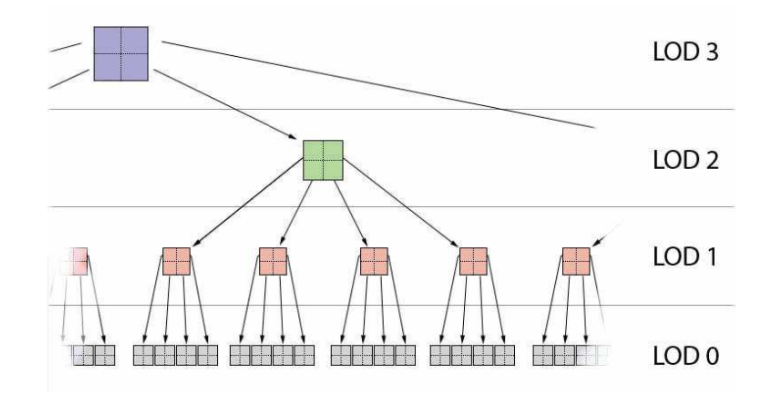
\includegraphics[scale = 0.8]{images/CDLOD1.png}
\caption{Niveaux de détails sur un quadtree}
\source{https://dept-info.labri.fr/~narbel/PdP/Subjects21-22/CLOD-Planets/cdlod_latest.pdf}
\end{figure}

\newpage

Ainsi, l'algorithme pourra simplement sélectionner les noeuds correspondant au bon niveau de détail en fonction de la position relative de l'utilisateur par rapport au maillage. Notamment, en utilisant la distance réelle entre l'observateur et les sommets du maillage, il est possible de représenter un nombre de points constant à l'écran et rendre l'algorithme plus prévisible, en théorie. Bien sûr, ces méthodes doivent être adaptées au fait que nous travaillons sur une surface sphérique et non plane, ce qui peut avoir des conséquences sur le calcul de distances et donc sur le rendu final.

Selon l'auteur, cette méthode permet de répondre à quelques défaillances des algorithmes de LOD classiques, et met en évidence des besoins qui pourront nous être utiles :

\begin{itemize}
    \item[-] En utilisant la distance réelle et non simplement la latitude/longitude de l'observateur, l'algorithme apporte plus de précision sur les niveaux de détail à afficher. Cet aspect est particulièrement important dans le cas d'une surface sphérique comme c'est le cas ici.
    \item[-] Il permet d'éviter l'apparition d'artefacts graphiques lors des transitions, car le maillage est complètement remplacé avant l'étape de transition.
    \item[-] En terme de performances : Les algorithmes classiques requièrent des calculs additionnels pour afficher des transitions fluides entre les différents niveaux de détail en créant des connexions (sommets) intermédiaires, ce qui n'est pas le cas pour l'algorithme CDLOD.
\end{itemize}

Au final, nous aurons à chaque frame du rendu une carte divisée en niveaux de détails dépendant de la position de l'utilisateur. Sur la figure 2.6, on remarque bien que la division s'affine d'un facteur 2 plus on se rapproche de l'observateur. La zone sombre représente les parties en dehors du champs de vision. 

\vspace{0.3cm}

\begin{figure}[h]
\centering
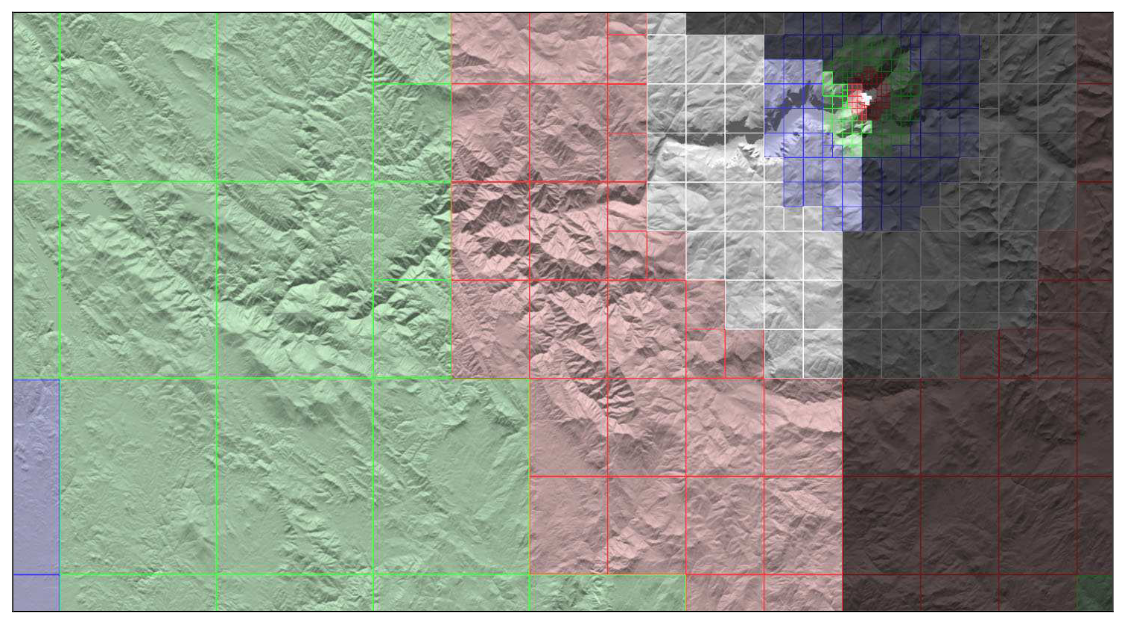
\includegraphics[scale = 0.6]{images/CDLOD2.PNG}
\caption{carte découpée en LOD}
\source{https://dept-info.labri.fr/~narbel/PdP/Subjects21-22/CLOD-Planets/cdlod_latest.pdf}
\end{figure}


Bibliothèque de gestion de quadtrees : https://github.com/dfriend21/quadtree

\newpage

\chapter{Description des besoins}

\section{Niveau de détail}

\textbf{Besoins Fonctionnels}

\begin{enumerate}
    \item \textbf{Lecture des heightmaps en entrée} : De manière générale, les heightmaps sont stockées dans des formats d'images standard car elles représentent une structure de valeurs en 2D, chaque pixel contenant la hauteur du terrain en ce point. Dans un premier temps, et dans un soucis de simplification, l'idéal serait de récupérer un fichier RAW contenant les données brutes de la heightmap codées en 16 ou 32 bits selon la précision nécessaire. Par la suite, nous pourrons étendre l'éventail des formats acceptés.
    
    \item \textbf{Algorithme CDLOD} :
    \begin{enumerate}
        \item La première étape de l'algorithme est le stockage de la heightmap sous forme de quadtree. Cette étape implique l'utilisation ou la création d'une bibliothèque de gestion de quadtrees. Celle-ci devra permettre au minimum la création et la suppression d'un arbre, l'ajout et la suppression de noeuds ainsi qu'une méthode de parcours de l'arbre.
        \item Dans un second temps, nous devons effectuer la sélection des noeuds du quadtree pour le rendu. Cette action est effectuée à chaque fois que l'observateur se déplace dans la scène, et donc possiblement à chaque frame. Pour savoir quels noeuds sont sélectionnés, les distances couvertes par chaque niveau de LOD sont pré-calculées (cf Partie 2.2 : \textit{Algorithmes de niveau de détail}). A chaque fois qu'un mouvement est détecté, l'algorithme recherche les noeuds représentant les parties du terrain actuellement visibles et le niveau de détail avec lequel elles doivent être tracées.
        \item Enfin, chaque noeud sélectionné doit être stocké dans une structure de données temporaire qui doit contenir sa position dans la scène, sa taille et son niveau de détail. D'autres informations peuvent y être ajoutées si elles sont nécessaires au rendu graphique.
    \end{enumerate}
    
    \item \textbf{Communication avec le module de rendu} : Comme nous pouvons le constater, les modules vont échanger une grande quantité d'informations et ce possiblement à chaque frame du rendu.
    
    \item \textbf{Visualisation OpenGL} :
    \begin{enumerate}
        \item \textbf{Fenêtre de visualisation} : 
            Création par programmation d'une fenêtre de visualisation qui interagit avec un objet de heightmap. La première étape pour utiliser OpenGL est de créer un context et généralement une fenêtre associée capable d'afficher un rendu OpenGL. Ces deux tâches seront effectuées par la bibliothèque GLFW. 
            \begin{itemize}
                \item \textbf{GLFW} est une bibliothèque Open Source multiplateforme pour le développement OpenGL sur le bureau. Il fournit une API simple pour créer des fenêtres, des contextes et des surfaces, recevoir des entrées et des événements.
            \end{itemize}
            \begin{figure}[h]
                \centering
                \includegraphics[scale = 0.5]{images/Exemple_de_fenêtre_de_visualisation_WSL2_XLaunch.png}
                \caption{Exemple de fenêtre de visualisation. WSL2. XLaunch.}
            \end{figure}
        \item \textbf{Création de la fonctionnalité nécessaire et intégration de l'existant pour un fonctionnement pratique de base} :
        Dans cette partie, nous allons utiliser deux bibliothèques : Eigen et Glbinding. 
        \begin{itemize}
            \item \textbf{Eigen} est une bibliothèque C++ d'algèbre linéaire. Elle sera utilisée pour la représentation et manipulation de matrices, vecteurs, transformations géométriques et résolution de systèmes d'équations.
            \item \textbf{Glbinding} exploite des fonctionnalités C++ 11 telles que les classes enum, les lambdas et les modèles variadiques, au lieu de s'appuyer sur des macros ; tous les symboles OpenGL sont de véritables fonctions et variables. Il fournit des paramètres de sécurité de type, des en-têtes d'API par fonctionnalité, une résolution de fonction paresseuse, une prise en charge multi-contextes et multi-threads, des rappels de fonctions globaux et locaux, des méta-informations sur la liaison OpenGL générée et le runtime OpenGL, ainsi que des outils et des exemples.
        \end{itemize}
        \item \textbf{Initialisation de la caméra} : 
        La portée de vue de la caméra et sa position décident des nœuds à dessiner et de la profondeur de la cascade des nœuds. Les nœuds les plus proches de la caméra sont en cascade jusqu'aux nœuds feuilles, dessinant une géométrie plus dense. La fonctionnalité de la caméra consiste à déplacer l'utilisateur sur une zone ou à modifier la distance de rendu d'un objet à l'aide des boutons. 
        \begin{itemize}
            \item PAGE UP : S'éloigner de l'objet
            \item PAGE DOWN : Se rapprocher de l'objet
            \item KEY UP : Tourner la caméra vers le haut
            \item KEY DOWN : Tourner la caméra vers le bas
            \item KEY LEFT : Tourner la caméra à gauche
            \item KEY RIGHT : Tourner la caméra à droite
            \item KEY W : définir le mode wireframe
            \item KEY E : activer / désactiver les mesh edges
            \item KEY + et KEY - : pour définir la plage de vues quadtree
        \end{itemize}
        
        \begin{figure}[h]
            \centering
            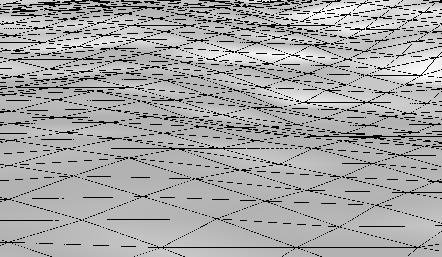
\includegraphics[scale = 0.7]{images/mesh_edges.png}
            \caption{Exemple de mesh edges.}
            \source{https://github.com/drecuk/QuadtreeTerrain}
        \end{figure}
         \begin{figure}[h]
            \centering
            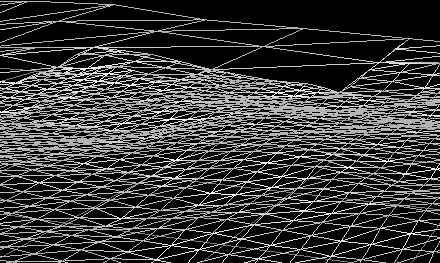
\includegraphics[scale = 0.7]{images/view_quadtree.png}
            \caption{Exemple de visualisation d'un Quadtree en mode wireframe}
            \source{https://github.com/drecuk/QuadtreeTerrain}
        \end{figure}
        \item \textbf{Créer une boîte à outils pour travailler avec des objets} :
        Après avoir traité le heightmap, il doit être installé sur la sphère. Les bibliothèques ObjFormat et tinyobjloader seront utilisées pour cela.
        \begin{itemize}
            \item \textbf{tinyobjloader et ObjFormat} sont des bibliothèques pour charger des maillages au format Wavefront OBJ.
        \end{itemize}
        \item \textbf{Chargement du RAW bitmap} :
        Le remplissage de la structure de données avec les données RAW bitmap de 8 bits pour chaque élément du tableau. Ce sont ces données qui seront utilisées pour visualiser le heightmap.
        \item \textbf{Implémentation logicielle de CDLOD} :
        La supclasse crée et maintient une structure quadtree. Chaque noeud de cette structure est décrit par la structure de noeud. ID et ParentID associent le noeud actuel au parent, et l'index de branche enregistre les ID des nœuds enfants. Ceci décrit les points à partir desquels les quads OpenGL sont construits (surface du terrain). Chaque nœud a 3 x 3 sommets, que notre constructeur utilise pour dessiner des triangles.
    \end{enumerate}
\end{enumerate}

\vspace{0.3cm}

\textbf{Besoins non-fonctionnels}

\textbf{Taille des données en mémoire} : L'implémentation pratique d'un logiciel de rendu de terrain doit tenir compte de la taille de ce dernier. Ici, il y a deux facteurs principaux à prendre en compte :
\begin{enumerate}
    \item \textbf{Les données de terrain} : Pour ne pas garder la totalité des données de la heightmap en mémoire, celle-ci peut-être divisée en blocks représentants les morceaux de terrain potentiellement visibles par l'observateur. Ces fragments peuvent être transmis sous forme de data-stream pendant le rendu. Cette méthode est d'autant plus efficace que l'algorithme CDLOD effectue déjà une sélection des blocks lors du calcul de LOD. 
    \item \textbf{Les données du quadtree} : Plus volumineux encore, les noeuds du quadtree contiennent des détails tels que la taille, la position, les voisins du noeud, etc... beaucoup d'informations qui peuvent être superflues pour l'étape de rendu. La version StreamingCDLOD de l'algorithme présenté dans le chapitre 2.2 évite ce problème en ne gardant que les valeurs minimales et maximales de la surface couverte par le noeud, qui sont stockées dans une matrice 2x2 pour chaque noeud. Le reste des données est automatiquement généré lors du parcours du quadtree.
    \item \textbf{Performance}: Le temps de traitement du programme ne dépasse pas quelques minutes.
    \item \textbf{Passage à l'échelle} : Lors de la création du quadtree ou dans la phase de rendu, s'assurer que le programme puisse gérer des heightmaps très grandes et très détaillées.
    \item \textbf{Visualisation OpenGL} :
    \begin{enumerate}
        \item \textbf{Performance:}
        \begin{enumerate}
            \item Le temps de traitement du programme ne dépasse pas quelques minutes.
            \item Garder un affichage fluide de rendu de heightmap.
        \end{enumerate}
            \item \textbf{Contraintes et difficulté techniques:}
            \begin{enumerate}
                \item Surface sphérique. L'ordinateur doit générer un maillage de base convexe pendant la génération du terrain.
                \item Utiliser un maillage de triangle équilatéraux plutôt que d'autres polygones.
            \end{enumerate}
        \item \textbf{Portabilité:}
        \begin{enumerate}
            \item Utiliser une machine contenant une carte graphique avec une version d'openGL de préférence openGL 3.3.
            \item Ajouter le contrôle de la molette de la souris au lieu de boutons, pour un contrôle plus facile de la caméra.
        \end{enumerate}
        \item \textbf{Contraintes d'affichage:}
        \begin{enumerate}
            \item Faire des tests pour pouvoir afficher un nombre conséquents de triangles.
            \item Récupérer la taille totale et restante de la mémoire du GPU avec GL NVX gpu memory info.
        \end{enumerate}
    \end{enumerate}
\end{enumerate}

Enfin, il est possible de compresser d'une part les heightmaps, et d'autre part les données des noeuds les plus détaillés du quadtree, en stockant les valeurs de la matrice min/max du noeud dans l'espace inutilisé de la matrice du noeud parent avec une faible perte de précision.

\chapter{Les scénarios d'utilisation}
\section{Scénario :}

\begin{enumerate}

\item[\sffamily 1.] Le client lance le fichier exécutable 
\item[\sffamily 2.] Un explorateur de fichier s'ouvre, demandant à l'utilisateur de spécifier l'emplacement d'une heightmap. Le logiciel va alors stocker cette heightmap sous forme de quadtree.
\item[\sffamily 3.] Une fenêtre graphique s'ouvre affichant le rendu placé sur le centre de la heighmap.
\item[\sffamily 4.] Le client dezoom via la molette de sa souris.
\item[\sffamily 5.] Le client se déplace sur la surface à l'aide des flèches de son clavier. 
\item[\sffamily 6.] Le client applique une rotation sur la planète en appuyant sur la touche R.
\item[\sffamily 7.] L'utilisateur choisit de changer de heightmap en appuyant sur la touche C.
\item[\sffamily 8.] L'utilisateur active le maillage en appuyant sur la touche M.
\item[\sffamily 9.] Le client choisit d'afficher des informations sur le programme en appuyant sur la touche H.
\item[\sffamily 10.] L'utilisateur met le programme en pause en appuyant sur P.
\item[\sffamily 11.] Le client quitte le logiciel en appuyant sur Q.



\end{enumerate}

\section{Extensions :}

\begin{enumerate}

\item[\sffamily 1a.] La configuration de l'appareil du client ne permet pas de  faire fonctionner notre logiciel.
\begin{itemize}
    \item Un message d'erreur s'affiche et le logiciel ne s'exécute pas.
\end{itemize}
\item[\sffamily 2a.] L'utilisateur ferme l'explorateur de fichier
\begin{itemize}
    \item Le logiciel se ferme
\end{itemize}
\item[\sffamily 2b.] Le client utilise le logiciel avec un fichier ne correspondant pas à une heightmap ou pas compatible avec notre implémentation.
\begin{itemize}
    \item Un message d'erreur s'affiche et le logiciel se ferme.
\end{itemize}

\end{enumerate}

\newpage

\chapter{Tests}

\section{Test Génération des heightmaps}
\begin{enumerate}
    \item Description : Vérifier que la heightmap générée est valide et pourra être lue par notre logiciel
    \item Données utilisées : 
    \begin{enumerate}
        \item Fichier vide
        \item Fichier non vide mais invalide
        \item Fichier non vide mais d'un type incorrect
        \item Fichier non vide de type correct mais avec des données corrompues
        \item Fichier correct, on pourra par exemple le générer avec la bibliothèque \cite{libnoisewebsite}
    \end{enumerate}
    
    Résultats attendus : Si le fichier est invalide le test doit échoué et afficher un message d'erreur contenant une description du problème.
\end{enumerate}

\section{Test Algorithme CDLOD}
\subsection{Génération d'un quadtree à partir d'une heightmap}
\begin{enumerate}
    \item Description : Vérifier la validité du quadtree suivant sa définition.
    \item Données utilisées :
    \begin{enumerate}
        \item Heightmap vide
        \item Heightmap non vide
        \item Autre fichier
        \item Heightmap corrompue
    \end{enumerate}
    \item Résultats attendus : Si la heightmap est vide alors le Quadtree doit l'être aussi, dans le cas contraire on vérifiera la validité du Quadtree généré
\end{enumerate}

\subsection{Sélection des noeuds pour le rendu}
\begin{enumerate}
    \item Description : Vérifier que la sélection des noeuds du quadtree se réalise correctement 
    \item Données utilisées :
    \begin{enumerate}
        \item Quadtree vide
        \item Quadtree non vide
    \end{enumerate}
    \item Résultats attendus : Si le quadtree est vide alors l'algorithme ne doit pas essayer de sélectionner de noeuds dans le cas contraire CDLOD doit nous renvoyez les noeuds correspondants et leurs niveau de détails
\end{enumerate}

\section{Test des interactions utilisateur}
\subsection{Zoom}
\begin{enumerate}
    \item Description : Opérer un zoom, observer le changement du niveau de détail (ou pas).
    \item Déroulement du test : Une fois que l'utilisateur a zoomé l'algorithme CDLOD doit nous envoyez les noeuds représentant les parties du terrains visibles et la fenêtre graphique doit se mettre à jour.
\end{enumerate}

\subsection{Activer le maillage}
\begin{enumerate}
    \item Description : Vérifier que si l'utilisateur active le maillage, celui-ci s'affiche à l'écran
    \item Déroulement du test : Une fois que l'utilisateur a activé le maillage, l'algorithme CDLOD doit nous envoyez les informations du quadtree courant : Sommets et arrêtes et la fenêtre graphique doit se mettre à jour.
\end{enumerate}

\subsection{Raccourcis clavier}
\begin{enumerate}
    \item Description : Vérifier qu'à chaque saisie d'un raccourci clavier pour se déplacer la fenêtre graphique se met à jour
    \item Déroulement du test : Une fois que l'utilisateur a saisi le raccourci clavier, on vérifie que la position de la caméra soit modifiée en accord avec les paramètres définis.
\end{enumerate}

\bibliography{biblio}
\bibliographystyle{alpha}

\end{document}
